%%% -*-LaTeX-*-

\chapter{Modern NICs}
\label{chap:modernnics}
Network Interface Cards have grown complex over time and present peculiar opportunities and 
challenges as part of a modern distributed system. It is imperative that today's
database system designer treats network transmission as a first class citizen in every design decision.
Previous research for optimising databases were focussed more on processing time spent on a 
database query~\cite{dbmsproctime}, but today's truth is that lion's share of the end-to-end latency
while processing a query is spent in network.
Since we are not reeling from slow disks anymore, the bulk of I/O bottleneck in a distributed system today is in network transmission.
Adding this to the fact that the modern NIC allows us to offload CPU from the data transfer path,
the saved memory bandwidth and CPU cycles could be utilised for useful work 

Network cards have had TCP offloading baked in as TCP Offload Engine for some time now, but it was getting 
more and more ineffective because of performance issues and complexities involved~\cite{tcpoffload}.
RDMA~\cite{rdmapatent,rdmacase,rdma} was proving to be a much better alternative with TCP offloading where
transport offloading was just one among varios benefits involved. Development of advanced switching 
interconnects such as PCI express~\cite{pcie} made it possible to develop highly performant 
network devices offering throughputs and latencies a couple of orders of magnitudes better
than what was possble with prior transports such as TCP. This chapter introduces the various design 
trade-offs we have to make and walks through the evaluation of those choices with the help of a microbenchmark.


\section{Zero Copy and Copy Out}
Kernel bypass is a ubiquitous feature in the modern NIC and key to accessing remote memory directly 
from across the network. While the literature defines kernel-bypass any data movement that doesn't 
involve copying between user space and kernel space, even packet capturing libraries~\cite{pcap} could fall
under those definitions. Newer network controllers make use of vectored I/O, otherwise known as scatter/gather I/O
where a single procedure reads data from multiple buffers and writes it to single buffer. The Mellanox Infiniband ConnectX\textregistered-3
NIC that we profiled provides a scatter/gather list which powers it's on NIC DMA engine. In this material, this specific kernel bypass
mechanism is what we are going to colloqially refer as Zero Copy.

Zero Copy should be christened in the context of traditional copy. Before kernel bypass became 
commonplace, the steps for copying data over the network using socket programming was as follows. 
The application calls a send function in a socket library and the data for sending is assembled 
in a transmit buffer, this transmit buffer is copied on to the on-NIC buffers and the data is 
send over the wire. We could employ the same technique in the kernel bypass capable NIC as well.
Instead of employing a multi entry scatter/gather list, the records could be assembled on 
to a temporary buffer and this buffer could be treated as a single entry scatter/gather list
and then transmitted over the network. We will be calling this technique \enquote{Copy Out} from now on.


Zero copy DMA facilitates a scatter gather list of buffer descriptors
which could be mapped to non contigous locations in memory on demand. These provide
the added benefit that network headers don't need to exist along with data and helps bring more flexibility 
in deciding the transport layer. One subtle thing to note here is that Zero Copy only implies the absence 
of a memcopy from the records to a buffer. The data still needs to be copied to the on-NIC buffers before 
it is sent out via the network cable. This is different from what happens when we call socket send on a traditional 
tcp stack where the data for transmission is pre assembled in a huge buffer and then copied across the network.
We evaluate how Zero Copy performs in contrast with the more traditional network copy approach reffered
 as Copy Out from now on.

\section{Memory Bandwidth}
Interestingly, the additional copy involved in the traditional approach hurts memory bandwidth of the system more than contributing 
to additional CPU load purely from the perspective of network transmission. Our evaluation show us that while the traditional
copy adds upto 25\% increase in absolute CPU utilisation, making use of the high throughput available in NICs by transmitting
near line rate takes up one fourth of the total available memory bandwidth in a modern server. We should read this in the context that 
network transmission is not the primary responsibility of a server in a distributed system. Most of the memory bandwidth wasted in 
just aggregating the data before transmission could be used as part of actual computation or other useful rearrangement of data in 
the query response. Chapter \ref{chap:impact} will fully discuss the impact on memory bandwidth and other parameters while the system 
is transmitting large amounts of data.


\section{NIC structures in detail}
\begin{figure}[t]
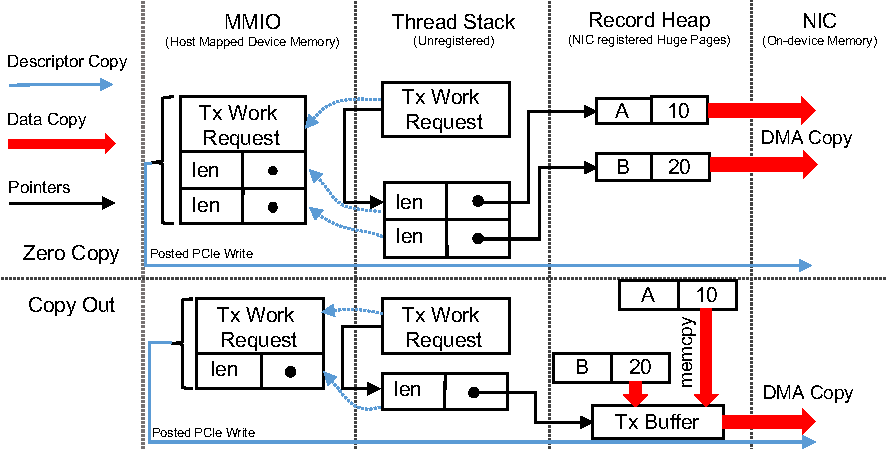
\includegraphics[width=\textwidth]{fig-mem-regions.pdf}
\caption{Key structures involved in network transmission.}
\label{fig:mem-regions}
\end{figure}

Figure~\ref{fig:mem-regions} details how an application interacts with a Mellanox
ConnectX-3\textregistered , a modern 56~Gbps NIC that uses kernel bypass. 
With zero-copy, transmit descriptors list several chunks of data for
the NIC to DMA. With copy-out, all data to be transmitted is first explicitly
copied into a transmit buffer by the host CPU; then, a transmit descriptor is
posted that references just the transmit buffer rather than the original
source data. Both zero-copy and the traditional copy-out approaches to transmission are shown.
In both cases the same three key data structures are involved. The first important structure is the
data to be transmitted, which lives in heap memory.  For zero-copy, the memory
where the records live must first be registered with the NIC. Registration
informs the NIC of the virtual-to-physical mapping of the heap pages. This is
required because the NIC must perform virtual-to-physical address translation
since the OS is not involved during transmission and the application has no
access to its own page tables.  Registration is done at startup and is often
done with physical memory backed by 1~GB hugepages to minimize on-NIC address
translation costs.

The second key structure is the descriptor that a thread must construct to
issue a transmission. With Mellanox NICs, a thread creates a work request and a
gather list on its stack. The work request indicates that the requested
operation is a transmission, and the gather list is a contiguous list of
base-bound pairs that indicate what data should be transmitted by the NIC (and
hence DMAed). For zero-copy, the gather list is as long as the number of chunks
that the host would like to transmit, up to a small limit. The NICs we use support
posting up to 32~chunks per transmit operation. Later, we find that this small
limit bottlenecks NIC transmit performance when chunks are small and numerous.

The final important structure is the control interface between the NIC and the
host CPU.  When the NIC is initially set up by the application, a region of the
NIC's memory is mapped into the application's virtual address space. The NIC
polls this region, and the host writes new descriptors to it from the thread's
stack to issue operations. The region is mapped as write-combining; filling a
cacheline in the region generates a cacheline-sized PCIe message to the NIC.
The NIC receives it, and it issues DMA operations to begin collecting the data
listed in the descriptor. The PCIe messages are posted writes, which means they
are asynchronous from the CPU's perspective. Even though PCIe latencies are much
higher than DRAM access, the CPU doesn't stall when posting descriptors, so the
exchange is very low overhead.

\subsection{Zero Copy vs Copy Out}
The key difference between zero-copy and copy-out is shown with the wide, red
arrows in Figure~\ref{fig:mem-regions}. Copy-out works much like conventional
kernel-based networking stacks: chunks of data are first copied into a single
transmit buffer in host memory. Then, a simple, single-entry descriptor is
posted to the NIC that DMAs the transmit buffer to an on-device buffer for transmission
As a result, copy-out requires an extra and explicit copy of the data, which is made
by the host CPU.  Making the copy uses host CPU cycles, consumes memory
bandwidth, and is pure overhead. Surprisingly, though, copy-out has
advantages including better performance when
records are small and scattered.  In those cases, complex gather descriptors
bottleneck the NIC, and using the host CPU to pre-assemble the responses can
improve performance.



\section{DDIO}
performance-oriented enhancements to the DMA mechanism have been introduced in 
Intel\textregistered Xeon E5 processors with their Data Direct I/O (DDIO)~\cite{ddio} feature,
allowing the DMA ``windows" to reside within CPU caches instead of system RAM. As a result,
CPU caches are used as the primary source and destination for I/O, 
allowing network interface controllers (NICs) to talk directly to the last level caches of local CPUs
and avoid costly fetching of the I/O data from system RAM. As a result,
DDIO reduces the overall I/O processing latency, allows processing of the I/O 
to be performed entirely in-cache and prevents the available memory bandwidth from becoming a performance bottleneck.
We fully investigate the effects of DDIO in Chapter~\ref{chapter:impact} in order to conclude the impact of 
traditional copy mechanisms.


\section{Inlining}
Mellanox NICs allow some data to be {\em inlined} inside the control message
sent to the NIC over PCIe. Our NICs allow up to 912~B to be included inside the
descriptor that is posted to the NIC control ring buffer.  Inlining can improve
messaging latency by eliminating the delay for the NIC to DMA the message data
from host DRAM, which can only happen after the NIC receives the descriptor.
Inlining benefits small request/response exchanges, but it does not help for
larger transmissions. This is because even though there is an extra delay
before the NIC receives the actual record data, that delay can be overlapped
with the DMA and transmission of other responses. Other researchers have shown
that sending data to the NIC via MMIO also wastes PCIe bandwidth~\cite{rdma}.
Almost all of our experiments have inlining disabled. Enabling inlining
gives almost identical throughput and overhead to copy-out, except it only
works for transmissions of ~912 B or less.


\section{Evaluation}
% TODO
% Should we put the tx buffers in huge pages?
% Knowing measured peak mem bw of our machines would be good, but it looks like
%   not all channels are populated?


\begin{table}[H]
\def\arraystretch{1.25}%  1 is the default, change whatever you need
\begin{tabular}{@{}l@{\hskip 12pt}l@{}}
\toprule
\textbf{CPU} & Intel Xeon E5-2450 (2.1~GHz, 2.9~GHz Turbo) \\
    & 8 cores, 2 hardware threads each \\
\textbf{RAM} & 16~GB DDR3 at 1600~MHz \\
\textbf{Network} & Mellanox MX354A ConnectX-3 Infiniband HCA (56 Gbps Full Duplex) \\
        & Connected via PCIExpress 3.0 x8 (63~Gbps Full Duplex) \\
%        & 7 Mellanox SX6036G FDR Switches \\
\textbf{Software} & CentOS 6.6, Linux 2.6.32, gcc 4.9.2, libibverbs 1.1.8, mlx4 1.0.6 \\
\bottomrule
\end{tabular}
\vspace{0.25eX}
\caption{Experimental cluster configuration.}
\label{tbl:config}
\end{table}



We explored hows the different designs trade-off database server efficiency and
performance, by building a simple model of an in-memory database system that
concentrates on data transfer rather than full query processing. In all experiments,
one node acts as a server and transmits results to 15 client nodes.
Our experiments were run on the Apt~\cite{Ricci+:OSR15} cluster of the
CloudLab~\cite{Cloudlab:URL} testbed: this testbed provides exclusive bare-metal
access to a large number of machines with RDMA-capable Infiniband NICs.
The proposed work that is pending will give more conclusive evidence for the 
Table~\ref{tbl:config} shows the Experiment Setup for the cluster where we profiled
the Mellanox Infiniband ConnectX-3 \textregistered NIC and impact of data layout and 
use of no update in place structures on transmission throughput. The cluster has 7
Mellanox SX6036G FDR switches arranged in two layers. The switching fabric is
oversubscribed and provides about 16~Gbps of bisection bandwidth per node
when congested. All of the experiments are
publicly available online\footnote{\url{https://github.com/utah-scs/ibv-bench}}.




\begin{figure}[t]
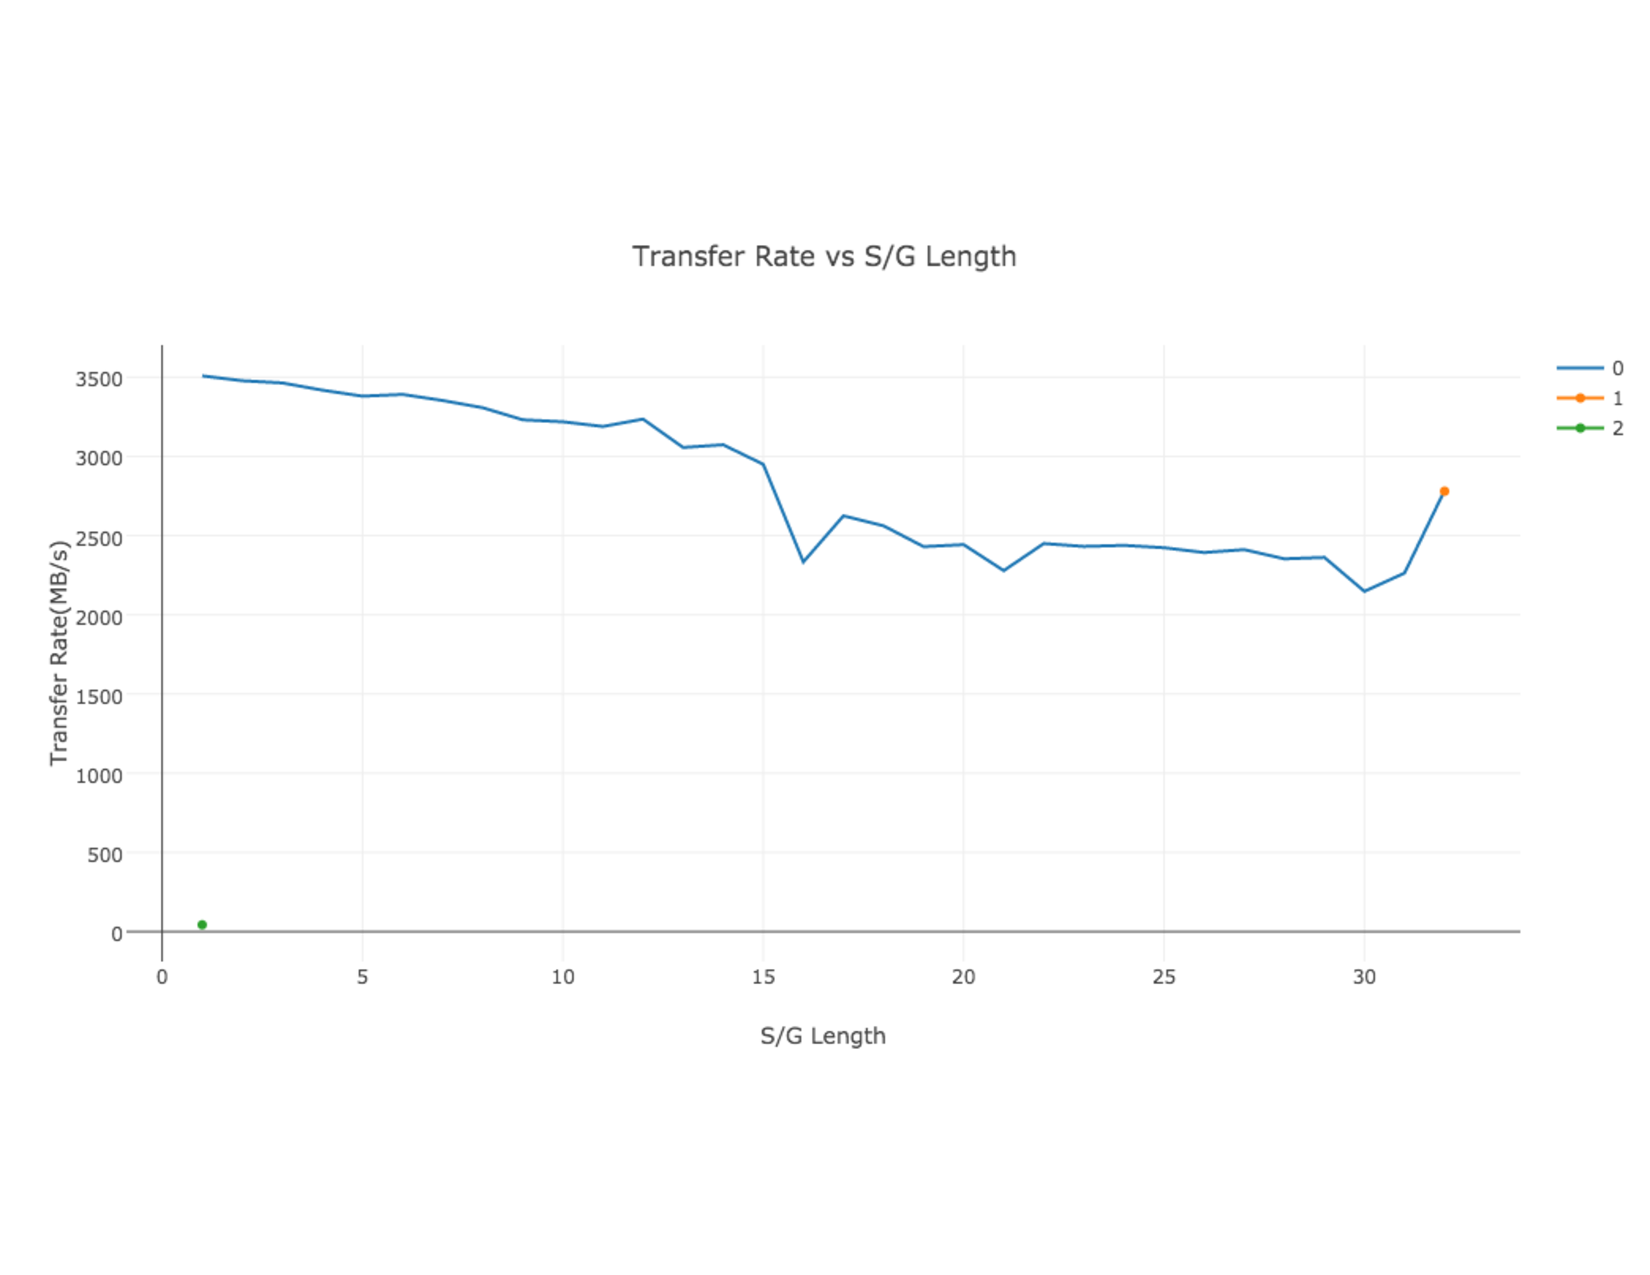
\includegraphics[width=\textwidth]{100B_transrate.pdf}
\caption{Transmission rate for 100 B records over different RDMA verbs and 
varying S/G lengths.}
\label{fig:100B_transrate}
\end{figure}

\begin{figure}[H]
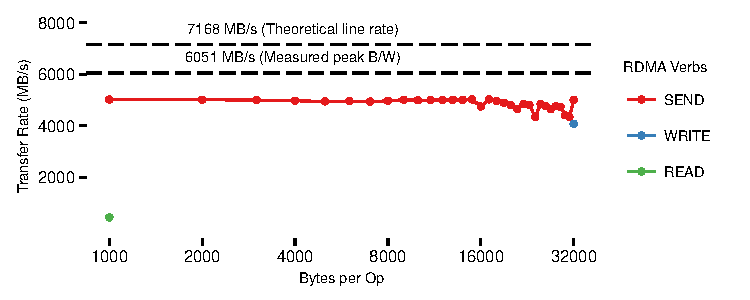
\includegraphics[width=\textwidth]{fig-1000B-RDMAverbs}
\caption{Transmission rate for 1000 B records over different RDMA verbs and 
varying S/G lengths.}
\label{fig:1000B_transrate}
\end{figure}


\subsection{RDMA modes}
We started out by getting measurements of transmission speeds using RDMA Reads.
We implemented rdma operations using infinibands ib verbs library. We implemented 
RDMA reads and write as op codes on the \cpp{ibv_send_wr} request which 
transmit data as \cpp{ibv_post_send} and also tried to measure the transmit
performance while using zero copy using \cpp{IBV_WR_SEND} as the operation.
We found that send operations can transmit multiple transmit buffer
It became evident quickly that one sided RDMA reads are not well positioned to 
take advantage of the zero copy paradigm since it only supports a remote read 
from a given location from the source. The rest of the experiments concerning
the impacts of NIC's impact on data layout were all done with send as the primary
operation. 


Figure~\ref{fig:100B_transrate} shows a comparison of transmission
peformance of various verbs transmitting 100 Byte records varying the number of records
that could be transmitted at a time for various operations.The green dot shows
the performance for RDMA reads which is also unfair
since RDMA reads can only transmit a single record at a time. The yellow dot
shows RDMA write performance. The modes shown was an enum of the format 
\cpp{enum Mode \{ MODE_SEND, MODE_WRITE, MODE_READ\}} and infiniband 
(\cpp{<infiniband/verbs.h>}) verbs library provides the  The record sizes were 
also an interesting measure to arrive at. It was obvious even from an earlier stage
that higher data sizes such as shown in Figure~\ref{fig:1000B_transrate} almost 
always results in better throughput measurements. In the world of In-memory databases,
there is an argument to be made that record sizes will be getting smaller since 
database designers can aggresively normalise and this has proven increasingly to
the liking of companies that manage large volumes of data in memory~\cite{fb-memcache,fb-workload}.


\subsection{Paging}
All our experiments transmit from a large region of memory backed by 4~KB pages
that contains all of the records. The region is also
registered with the NIC, which has to do virtual-to-physical address
translation to DMA records for transmission.
In some cases, using 1~GB hugepages reduces translation look aside buffer
(TLB) misses. We have realised that the NIC can benefit from
hugepages as well, since large page tables can result in additional
DMA operations to host memory during address translation~\cite{farm,rdma}. For
our experiments, the reach of the NIC's virtual-to-physical mapping is
sufficient, and hugepages have no impact on the results.


To explore how different designs trade-off database server efficiency and
performance, we built a simple model of an in-memory database system that
concentrates on data transfer rather than full query processing.  In all experiments, one node acts
as a server and transmits results to 15~client nodes.

Experiments transmit from a large region of memory backed by 4~KB pages that contains all of
the records.  The region is also
registered with the NIC, which has to do virtual-to-physical address
translation to DMA records for transmission.
In some cases, using 1~GB hugepages reduces translation look aside buffer
(TLB) misses.  The NIC can benefit from
hugepages as well, since large page tables can result in additional
DMA operations to host memory during address translation~\cite{farm,rdma}.  For
our experiments, the reach of the NIC's virtual-to-physical mapping is
sufficient, and hugepages have no impact on the results.

\subsection{Zero-copy Performance}
\label{sec:zero-copy-tput}

% stutsman: some old dead text, probably totally worthless.
% At some point make sure the rest of the text contains all of these ideas
% already.
%
% Smaller transmissions require more NIC interaction and PCI Express (PCIe)
% writes to transmit query results, but they can deal with discontinuous
% in-memory data layouts. In the case of zero-copy transmission, smaller
% transmissions may also reduce the amount of time that the database must keep
% records stable for the NIC.  Larger transmissions can also accommodate
% discontinuity through two different methods: copy-out or zero-copy, but
% discontinuity results in increased transmit descriptor size and complexity.

The first key question is understanding how database record layout affects the
performance of the transmission of query results.  The transmission of large
result sets presents a number of complex choices that affect
database layout and design as well as NIC parameters.  Range query
results can be transmitted in small batches or large batches and either via
copy-out or zero-copy.

To understand these trade-offs, we measure the aggregate transmission
throughput of a server to its 15~clients under several
configurations.  In each experiment, the record size, $s$, is either 1024~B or
128~B. Given a set of records that must be transmitted, they are then grouped
for transmission. For zero-copy, an $n$ entry DMA gather descriptor is created
to transmit those records where $ns$ bytes are transmitted per NIC transmit
operation. For copy-out, each of the $n$ records is copied into a single
transmit buffer that is associated with a transmit descriptor that only points
to the single transmit buffer. Each transmission still sends exactly $ns$
bytes, but copy-out first requires $ns$ bytes to be copied into the transmit buffer.
Intuitively, larger groups of records (larger sends) result in less host-to-NIC
interaction, which reduces host load and can increase throughput; the benefits
depend on the specific configuration and are explored below.

\begin{figure}[t]
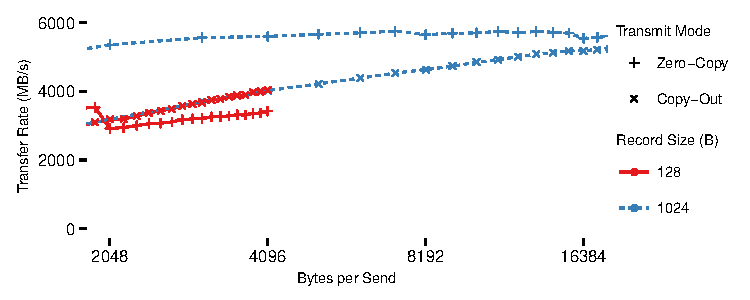
\includegraphics{fig-zero-copy-tput.pdf}
\caption{Transmission throughput for Zero Copy and Copy Out.}
\label{fig:zero-copy-tput}
\end{figure}

Figure~\ref{fig:zero-copy-tput} shows how each of these configurations impact
transmission throughput. For larger 1024~B records, using the NIC's DMA engine
for zero-copy shows clear benefits (aside from CPU and memory bandwidth
savings, which we explore in \S\ref{sec:overhead}). The database server is able
to saturate the network with zero-copy so long as it can post 6 or more
records per transmit operation to the NIC (that is, if it sends 6~KB or larger
messages at a time).

The figure also shows that using copy-out with 1024~B records, the NIC can also
saturate the network, but records must be packed into buffers of 16~KB or more.
This is significant, since it determines the transmission
throughput of the database when range queries only return a few
results. In this case, the DMA engine could provide a throughput boost
of up to 29\% over copy-out, but the benefit is specific to
that scenario. If range scans return even just 16 records per query, the
throughput benefits of zero-copy are almost eliminated.
% computePctTputImprovementForZeroCopy(loadMerged())
% [1] "128 B item pct improvement in tput for zero-copy"
%  [1]   8.105552  10.928705  14.097586  18.910805  28.721654  43.346138  51.993156  44.439383  55.446378
% [10]  43.414034  35.736397  26.654478  23.842016  20.787579  18.376618  -5.310453  -2.382863  -4.469114
% [19]  -5.565349  -6.927329  -6.270677  -7.919818  -8.681226  -9.356702 -11.269678 -11.943183 -12.265026
% [28] -13.209408 -13.396745 -13.930867 -14.057826 -12.286999
% [1] "Max 55.4463782269341"
% [1] "1024 B item pct improvement in tput for zero-copy"
%  [1] 53.841302 86.064417 55.299614 40.553317 37.989062 33.750689 30.841420 23.594658 21.917508 19.037890
% [11] 18.186771 15.621109 14.475694 12.246097 11.008283  7.318041  7.586871  7.262891  7.572221  7.396499
% [21]  7.427524  7.109614  7.039692  6.980079  6.610857  5.824279  5.979297  5.631181  5.694890  5.299445
% [31]  5.746029  5.610679
% [1] "Max 86.0644167799178"

Next, we consider 128~B records. The decreased access latency of
in-memory databases makes them well-suited to smaller, finer-grained records
than were previously common. One expectation is that this will drive databases
toward more aggressively normalized layouts with small records. This
seems to be increasingly the case as records of a few hundreds bytes or less
are now typical~\cite{fb-memcache,fb-workload}.

Figure~\ref{fig:zero-copy-tput} shows that for small 128~B records, the NIC DMA
engine provides little throughput benefit. Our NIC is limited to gather lists
of 32~entries, which is insufficient to saturate the network with such a small
record size. Transmission peaks at 3.5~GB/s.
Copying 128~B records on-the-fly can significantly outperform
zero-copy transmission when there are enough results to group per transmission.
In fact, copy-out can saturate the network with small records, and it
performs identically to copy-out with larger 1024~B records. We later discovered 
that the use of thread local storage in the benchmarks and more fine-grained locking 
in our own implementation produces a slightly different result showing a more 
conspicous improvement of zerocopy. We will discuss this
in detail in Chapter~\ref{chap:impact}. The rest of this material discusses the 
updated numbers when using thread local storage and more fine grained locking.

\subsubsection{Zero-copy Savings}
\label{sec:overhead}

\begin{figure}[H]
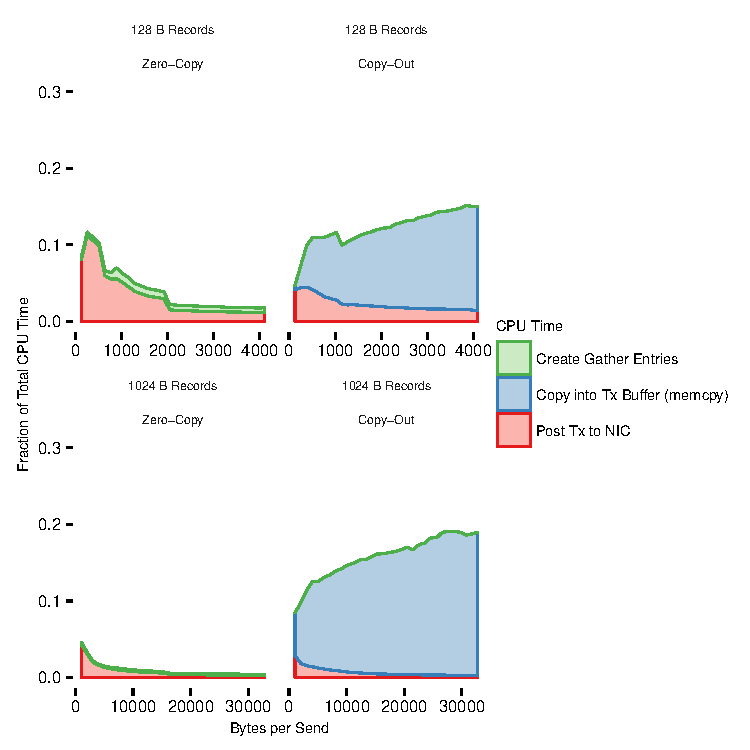
\includegraphics{fig-overheads.pdf}
\caption{Breakdown of absolute CPU overheads for transmission.}
\label{fig:overheads}
\end{figure}

In addition to improved performance, a goal of zero-copy DMA is to mitigate
server-side CPU and memory load. Figure~\ref{fig:overheads} breaks down
CPU time for all the scenarios; small and large records using Zero Copy and Copy-Out. We can observer that in the case 
of zero copy, most of the server CPU time is spent idling waiting for the NIC 
to complete transmissions. It is also obvious that that zero-copy always reduces 
the CPU load of the server, and, as expected, the effect is larger for larger records. 
With 1024~B records, the \memcpy  step of copy-out uses a maximum of 18\% CPU cycles 
of which 

Zero-copy eliminates copy overhead, but it adds overhead to create
larger transmit descriptors.  Each gather entry adds
16~B to the descriptor that is posted to the NIC.
These entries are considerable in size compared to
small records, and they are copied twice. The gather list
is first staged on the thread's stack and passed to the userlevel NIC driver. Next,
the driver makes a posted PCIe write by copying the descriptor (including the
gather entry) into a memory-mapped device buffer.  For large records,
constructing the list uses between 1~and~4\% of total CPU time, so zero-copy
saves about 3~to~6\% of CPU time over copy-out.

The memory bandwidth savings for zero-copy are more substantial.
Figure~\ref{fig:zero-copy-tput} shows that copy-out transmit performance nearly
matches zero-copy (5.6~GB/s versus 5.8~GB/s). Copy-out introduces exactly one
extra copy of the data, and \memcpy  reads each cache line once and writes it
once. So, copy-out increases memory bandwidth consumption
by 2$\times$ the transmit rate of the NIC or 11.2~GB/s in the worst case.  This
accounts for about 32\% of the available memory bandwidth for the machine that we used. Whether
using zero-copy or copy-out, the NIC must
copy data from main memory, across the PCIe bus, to its own buffers, which
uses another 6~GB/s of memory bandwidth.

% Need to know how much memory bw \memcpy/  actually burns.
% Based on pcm-memory.x and the membench tool I stuff in the ibv-bench
% directory \memcpy/  does one read and one write for each cache line it copies,
% probably at least when the copies are larger enough.
% Based on Erik's work it looks like row-buffers are 8 KB! Wow, this might
% actually impact our story in terms of energy efficiency!

For smaller 128~B records, the CPU and memory bandwidth savings are nearly the
same as for larger records.  In this case, copy-out uses up to 10.8\% of the
CPU cycles on the socket, and zero-copy uses 5.5\%.  Eliminating the extra
\memcpy/  halves CPU overhead for transmission; a savings of about 5\% of the
total socket's CPU cycles.  Just as before, the memory bandwidth savings is
twice the transmission rate or 11.2~GB/s.  Overall, this makes copy-out
reasonable for small records scattered throughout memory, especially since zero-copy cannot saturate the network in these cases (\S\ref{sec:zero-copy-tput}).

\begin{figure}[H]
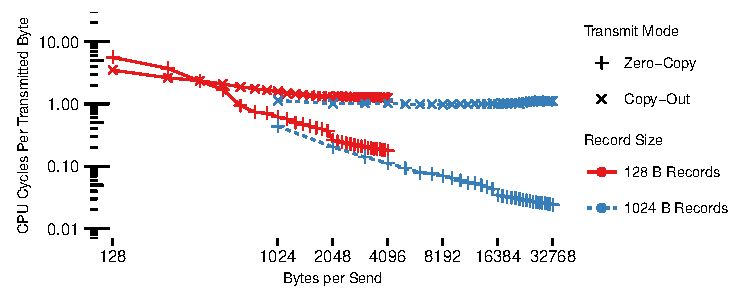
\includegraphics{fig-cycles.pdf}
\caption{Cycles per transmitted byte for large and small records with zero-copy and copy-out. Note the log-scale axes.}
\label{fig:cycles}
\end{figure}

The results break down where the CPU and memory bandwidth savings come from,
but not all configurations result in the same transmit performance. For
example, Figure~\ref{fig:zero-copy-tput} shows that when transmitting
128~B~records, copy-out gets up to 53\% better throughput than zero-copy. As a result,
minimizing CPU overhead can come at the expense of transmit
performance.  The real efficiency of the server in transmission is shown in
Figure~\ref{fig:cycles}. The figure shows how many cycles of work the CPU does
to transmit a byte in each of the configurations, which reveals two key things.
First, it shows that, though the absolute savings in total CPU cycles is small
for zero-copy, it does reduce CPU overhead due to transmission by up to 76\%.
Second, the improvement is a modest 12\% for small records, since
copy-out can transmit in larger, more efficient batches.

% LMBench 3.0 Memory Results from our Machines
% *Local* Communication bandwidths in MB/s - bigger is better
% -----------------------------------------------------------------------------
%  Host                OS  Pipe AF    TCP  File   Mmap  Bcopy  Bcopy  Mem   Mem
%                               UNIX      reread reread (libc) (hand) read write
% --------- ------------- ---- ---- ---- ------ ------ ------ ------ ---- -----
% node-0.st Linux 2.6.32-                              4813.3 5606.8 8349 6797.
%

% Copy 512 MB between two regions of a single hugepage 100 times.
% One process at a time:
% [stutsman@node-0 ~]$ ./membench
% CPU Secs 12.023564
% bw 4.158501 GB/cpuS
%
% 8 processes at a time:
% [stutsman@node-0 ~]$ CPU Secs 49.799340
% bw 1.004029 GB/cpuS
% CPU Secs 49.842697
% bw 1.003156 GB/cpuS
% CPU Secs 49.905588
% bw 1.001892 GB/cpuS
% CPU Secs 50.420696
% bw 0.991656 GB/cpuS
% CPU Secs 50.585852
% bw 0.988419 GB/cpuS
% CPU Secs 50.699039
% bw 0.986212 GB/cpuS
% CPU Secs 50.757823
% bw 0.985070 GB/cpuS
% CPU Secs 50.850676
% bw 0.983271 GB/cpuS

% > sum(d[d$chunkSize == 128 & d$chunksPerMessage == 64,]$mbs)
% [1] 4438.671


